  \documentclass[11pt,a4paper,sans]{moderncv}
  \moderncvstyle{banking}
  \moderncvcolor{black}
  \nopagenumbers{}

  \usepackage[utf8]{inputenc}
  \usepackage[top=0.30cm, bottom=0.30cm, left=0.50cm, right=0.50cm]{geometry}
  \usepackage{ragged2e}
  \usepackage{multicol}
  \usepackage{enumitem}
  \usepackage{amssymb}
  \usepackage{fontawesome5}
  \usepackage{xcolor}
  \usepackage{hyperref}
  \hypersetup{colorlinks=true, urlcolor=black}

  % Custom cventry
  \newcommand*{\customcventry}[7][.10em]{%
  \begin{tabular}{@{}l}
      {\bfseries #4} \\
      {\itshape #3}
  \end{tabular}
  \hfill
  \begin{tabular}{l@{}}
      {\bfseries #5} \\
      {\itshape #2}
  \end{tabular}
  \ifx&#7&%
  \else{\\
  \begin{minipage}{\maincolumnwidth}%
      \footnotesize#7%
  \end{minipage}}\fi%
  \par\addvspace{#1}
  }

  \begin{document}

  % Ultra-compact header: photo left (not in margin), title/info centered and bigger
  \hspace*{0.03\textwidth}% less horizontal space before photo (10% bump back)
  \begin{minipage}[c]{0.13\textwidth}
    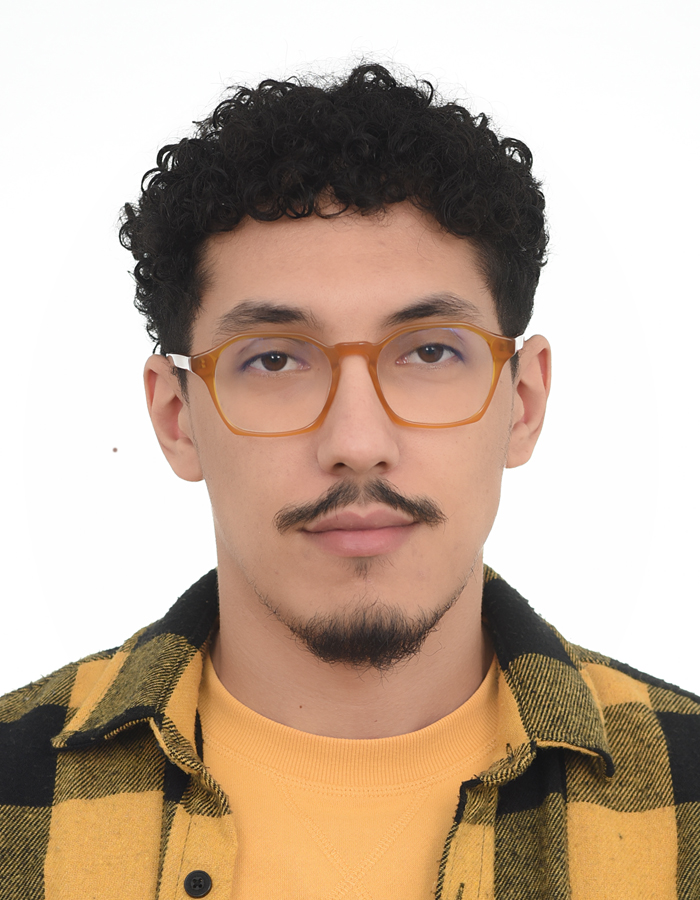
\includegraphics[width=0.85\linewidth]{images/ahmed.jpg}
  \end{minipage}%
  \hfill
  \begin{minipage}[c]{0.84\textwidth}
    \begin{center}
      {\fontsize{20}{22}\selectfont\textbf{Ahmed MAKROUM}}\\[0.7em]
      {\fontsize{13.2}{15.4}\selectfont  Data Engineer – Big Data \& Cloud} \\[0.5em] % <--- Ajouté ici
      {\fontsize{10.5}{12.3}\selectfont
        \faMobile\enspace +212 6 64 71 62 19 \quad
        \faEnvelope\enspace ahmedmakroum3@gmail.com \quad
        \faHome\enspace Casablanca, Maroc \
        \faLinkedin\enspace \href{https://www.linkedin.com/in/ahmed-makroum/}{in/ahmed-makroum} \quad
        \faGithub\enspace \href{https://github.com/ahmedmakroum}{github.com/ahmedmakroum}\quad
        \faGlobe\enspace \href{https://makroum.website}{makroum.website}
      }\\[1em]
    \end{center}
  \end{minipage}
  \vspace{-11pt}

  % PROFIL
  \section{\fontsize{11}\selectfont Profil}
  \vspace{-6pt}
Ingénieur d’état spécialisé en data engineering, avec une pratique concrète de la création de pipelines de données, de systèmes d’ingestion et de transformation, et de l’utilisation de plateformes cloud. Je cherche à rejoindre une équipe où je pourrai concevoir des architectures de données fiables, en améliorer la performance, tout en continuant à affiner mes compétences à travers des projets exigeants.
  % EXPÉRIENCE
  \vspace{-14pt}
  {\renewcommand{\labelitemi}{\raisebox{0.2ex}{\scalebox{1.15}{$\bullet$}}} % +15% size for bullets here only
  \section{\fontsize{11}\selectfont Expérience}
  \vspace{-3pt}

  
  \customcventry{09/2025 ‐ present}{\href{https://metave.ma/}{Metaverse}}{Data Engineer}{}{}{
  \begin{itemize}[leftmargin=0.6cm, itemsep=-2pt, topsep=0pt, partopsep=0pt, parsep=0pt]
  \fontsize{11}{12.3}\selectfont
     \item Créé des plans d’infrastructure data pour des clients avec GCP, AWS et des systèmes internes, facilitant la mise en place et l’uniformité des projets  
     \item Mis en place l’automatisation des déploiements avec Terraform, réduisant le travail manuel et rendant les environnements plus faciles à gérer et à étendre 
  \end{itemize}}


  \customcventry{03/2025 ‐ 08/2025}{\href{https://www.allianz.ma}{Allianz Maroc}}{Stage - Data Engineer}{}{}{
  \begin{itemize}[leftmargin=0.6cm, itemsep=-2pt, topsep=0pt, partopsep=0pt, parsep=0pt]
  \fontsize{11}{12.3}\selectfont
                \item Conçu et déployé des pipelines de données (NiFi, Spark) pour extraire, nettoyer et charger les données des systèmes d’assurance internes, automatisant un traitement auparavant manuel
                \item Intégré des sources fragmentées dans un entrepôt PostgreSQL, consolidant plusieurs flux métiers
                \item Créé des dashboards avec Metabase, facilitant l’accès aux données et la visualisation directe des indicateurs clé pour les utilisateurs métiers
                \item Développé et maintenu une application web de gestion des règlements de santé en architecture microservices (Spring Boot, Next.js), assurant une gestion fine des rôles et une authentification sécurisée, utilisée quotidiennement par les équipes métier
  \end{itemize}}

  \customcventry{06/2024 ‐ 08/2024}{\href{https://boti.education/}{BOTI School}}{Stage - Data Engineer}{}{}{
  \begin{itemize}[leftmargin=0.6cm, itemsep=-2pt, topsep=0pt, partopsep=0pt, parsep=0pt]
  \fontsize{11}{12.3}\selectfont
                \item Conçu et déployé un pipeline ETL distribué avec Apache Beam sur Google Cloud, capable de traiter des millions de logs utilisateurs de manière fiable et performante.  
                \item Structuré et optimisé des données issues de buckets GCP, permettant une analyse comportementale exploitable
                \item Développé des dashboards automatisés via Looker, adoptés par l’équipe pour soutenir les décisions stratégiques
  \end{itemize}}

  \customcventry{06/2023 ‐ 08/2023}{\href{https://6solutions.com/}{6solutions}}{Stage - Web and Mobile Developer}{}{}{
  \begin{itemize}[leftmargin=0.6cm, itemsep=-2pt, topsep=0pt, partopsep=0pt, parsep=0pt]
  \fontsize{11}{12.3}\selectfont
                \item Développé une plateforme de consulting multi-services (juridique, médical, financier), offrant une solution centralisée pour différents besoins clients 
                \item Réalisé le front-end avec Angular et le back-end avec Spring Boot, assurant une architecture web cohérente
                \item Conçu et déployé la version mobile de l’application en Flutter, permettant un accès fluide aux services depuis n’importe quel appareil
  \end{itemize}}

  \customcventry{07/2022 ‐ 08/2022}{\href{https://estatmar.ma/}{Finso}}{Stage - Game Developer}{}{}{%
  \begin{itemize}[leftmargin=0.6cm, itemsep=-2pt, topsep=0pt, partopsep=0pt, parsep=0pt]
  \fontsize{11}{12.3}\selectfont
                \item Développé un jeu éducatif ludique pour enfants, introduisant des notions de gestion et de stratégie de manière interactive 
                \item Réalisé le projet sous Unity, avec gameplay interactif, animations soignées et interface adaptée, assurant une expérience engageante pour le jeune public
  \end{itemize}}}
  

  % FORMATION
  \vspace{-11pt}
  \section{\fontsize{11}\selectfont Formation}
  \vspace{-4pt}
\noindent
\parbox[t]{0.78\textwidth}{
    \textbf{\href{https://emsi.ma}{EMSI – École Marocaine des Sciences de l’Ingénieur}}, \\
    Diplôme d’Ingénieur d'état en Informatique et Réseaux, option MIAGE 
    (Méthodes Informatiques Appliquées à la Gestion des Entreprises)
}
\hfill
\parbox[t]{0.2\textwidth}{
    \raggedleft \textit{09/2020 - 03/2025}
}
\vspace{0.3em}



{}

  % CERTIFICATIONS
  \vspace{-11pt}
  \section{\fontsize{11}\selectfont Certifications}
  \vspace{-5pt}
  \textit{Certifications obtenues via Coursera.}
  \begin{itemize}[leftmargin=0cm, itemsep=-2pt, topsep=0pt, partopsep=0pt, parsep=0pt, label={}]
      \item \textbf{\href{https://www.coursera.org/account/accomplishments/verify/G178XXP17WQA}{Machine Learning with Python}} (IBM)
      \item \textbf{\href{https://www.coursera.org/account/accomplishments/records/M5RKGX36BAVA}{IBM Data Engineering}} (IBM)
      \item \textbf{\href{https://google.com}{Building Scalable Java Microservices with Spring Boot and Spring Cloud}} (Google Cloud)
      \item \textbf{\href{https://www.coursera.org/account/accomplishments/verify/EK5SJM3YM7PX}{Introduction to Big Data with Spark and Hadoop}} (IBM)
      \item \textbf{\href{https://www.coursera.org/account/accomplishments/specialization/B4RCUAYCUG49}{Python for Everybody Specialization}} (University of Michigan)
      \item \textbf{\href{https://www.coursera.org/account/accomplishments/records/G867SJLRFQS2}{Google Business Intelligence}} (Google)
  \end{itemize}

  % COMPÉTENCES
  \vspace{-11pt}
  \section{\fontsize{11}\selectfont Compétences}
  \vspace{-6pt}
  \begin{itemize}[leftmargin=0cm, itemsep=-2pt, topsep=0pt, partopsep=0pt, parsep=0pt, label={}]
    \item \textbf{Data Engineering & Cloud:} : ETL, Big Data (Hadoop, Spark), Kafka • GCP, AWS, Docker, Terraform, CI/CD, Linux
    \item \textbf{Programmation & Données:} : Python, SQL, Java • PostgreSQL, MongoDB, Cassandra
    \item \textbf{Soft Skills} : Travail d’équipe, communication, adaptabilité, résolution de problèmes
  \end{itemize} 

 

  \end{document}

